\documentclass[11pt]{article}
\usepackage{cite}
\usepackage{amssymb}
\usepackage{amsmath}
\usepackage{graphicx}

\begin{document}

\title{Voronoi Diagrams to Evaluate Pass Reception}
\author{Christian Parker cxp220034@utdallas.edu}
\date{}
\maketitle

\begin{abstract}
    Voronoi diagrams are quite popular for evaluating field position in a number of sports such as soccer, basketball, and football. However, there are no methods for using them to
    evaluate pass reception. In this paper, we consider the use of Voronoi diagrams to evaluate pass reception. We construct a method that uses a two-dimensional Voronoi diagram,
    bounded by a rectangular field, to determine which player will receive a pass first. The method follows the path of the ball through each cell of the diagram and checks if the player
    in the cell can reach the ball before it exits. If there is a valid receiver, the method finds them in \(O(n)\) where \(n\) is the number of players on the field.
\end{abstract}

\section*{Introduction}
\paragraph{Problem Statement}
\begin{center}
    Given a set of points (the players), a speed for these points (how fast the players can run),
    and a parametric equation (the path of the ball), which of the players will intersect the ball first?
\end{center}

\paragraph{Assumptions}
\begin{enumerate}
    \item The players have no initial speed.
    \item The players can instantaneously reach full speed.
    \item Only two dimensions will be considered. We will not consider the possibility of passes over the players' heads.
    \item The receiver will always take the optimal path to the ball.
    \item The ball never intersects with a Voronoi vertex.
\end{enumerate}
These assumptions limit the scope of the problem, but also make the problem more manageable given the time constraints of this paper.
The solution is still highly relevant to sports where players frequently pass a ball along the same plane they are occupying (e.g. soccer, hockey, lacrosse, ultimate frisbee).
However, it may be less relevant to sports that frequently involve passes over players (e.g. football, basketball).

\subsection*{Related Works}
Voronoi diagrams seem to first be used to analyze soccer in a paper published in 2000 on \textit{Visualization of Dominant Region in Team Games and Its Application to Teamwork Analysis}.
The authors consider Voronoi diagrams briefly before defining and analyzing a new diagram that they call a dominant diagram~\cite{taki2000}. The dominant
diagram consists of dominance regions which are similar to the Voronoi cells but also take into account a player's initial velocity and acceleration.
From 2012 to 2023, at least three papers follow up on the idea of Voronoi diagrams for sports by acquiring real world data from soccer, futsal, and basketball.
They generate Voronoi diagrams for the data and examine how players control space and what spaces are valuable to scoring~\cite{Higgins_2023, FONSECA20121652, Bornn2016NBACR}.
There are also numerous blog posts that analyze sports (mostly soccer) using Voronoi diagrams in the same manner as these papers. However, they generally rely on handcrafted data rather
than data acquired from teams or leagues.

From here, several papers extend or modify Voronoi and dominant diagrams to evaluate space control in sports.
Two papers from 2016 and 2017 evaluate the quality of a pass based on the space controlled by each team before and after the pass is made.
In \textit{Evaluation of changes in space control due to passing behavior in elite soccer using Voronoi-cells}, the authors evaluate the quality of a pass based on the difference
in space control between the two teams on a soccer field. They only consider control over the attacking area, or the space within 30m of the goal. Control is calculated before
and after the pass and they find that attackers gain the most control when passing forward from midfield and passing within the attacking area~\cite{Rein2016}.
In \textit{Classification of Passes in Football Matches using Spatiotemporal Data}, the authors don't use dominant regions directly but instead use an approximation algorithm
to construct a dominant diagram. From this diagram, they extract some features for a machine learning model which then learns to classify passes as good or bad~\cite{Chawla_2017}.

The author of \textit{The Voronoi Diagram in Soccer} takes the perspective that dominance space diagrams aren't useful unless they consider the kinematics of a player. With this in mind,
they formulate a method to calculate dominant space of players given initial velocity, acceleration, top speed, and reaction time~\cite{efthimiou2022voronoi}.
In \textit{Football player dominant region determined by a novel model based on instantaneous kinematics variables}, another set of authors go one step further by using kinematic data collected
from real players to formulate a model for finding dominant regions~\cite{Caetano2021}.

In \textit{An approximate computation of the dominant region diagram for the real-time analysis of group behaviors}, the authors describe a method for constructing
dominant diagrams in real time for use in robot soccer. This paper does define a method for using the diagram to evaluate pass completion. However, the method
involves calculating the dominant diagram at every time step and then checking if the ball is in any region at that time. Therefore, the runtime is high
and the method is prone to error if the time step is too large~\cite{Nakanishi2010}.

While a few papers consider passing, none of them propose using Voronoi diagrams or dominant diagrams for determining the first possible point and time of pass reception.

\subsection*{Why Voronoi Diagrams?}
The advantage of a Voronoi diagram for this problem is that we can construct the diagram once and then rapidly test multiple paths for the ball.
The diagram is also a valuable visual reference from which players, coaches, or analysts can extract information.
In addition, Voronoi diagrams are already used in sports analysis, so this method fits nicely on top of analysis already being done.

\section*{Playing Field to Voronoi Diagram}
\subsection*{The Field}
We represent the field as a rectangle of size 120yds by 50yds. This is close enough to the size of a typical football or soccer field for our considerations.
We could also consider any other sports field by simply changing these dimensions to the regulation size for that sport.
The space of the field will be all points in \([0,50] \times [0,120]\).

\begin{equation}
    S := \{(x,y) \in \mathbb{R}^2 \ |\ 0 \leq x \leq 50, 0 \leq y \leq 120\}
\end{equation}

\subsection*{The Players}
The players will be represented as points within \(S\) and will be denoted by \(P\). The number of players on the field will be denoted by \(n\).
An example of players plotted on a field are shown in Figure~\ref{fig:field}.

\begin{equation}
    P = \{p_1, ..., p_n\} \subset S
\end{equation}

\noindent We assume that all players have the same speed of \(8 yds/sec\). This is based on data observed in
\textit{Influence of Players' Maximum Running Speed on the Team's Ranking Position at the End of the Spanish LaLiga}~\cite{delcoso2020influence}.
In 2020, they found that, for the 475 players tracked across the 2017-2018 season, the average max speed was \(~30.7 \pm 0.6 km/h\) or \(~9.3 yds/sec\).
Since players likely only hit their max speed a few times a game, we propose \(8 yds/sec\) as a more realistic speed to receive the average pass.

\begin{equation}
    v(p_i) = 8 yds/sec
\end{equation}

\begin{figure}[h]
    \centering
    \begin{minipage}{0.45\textwidth}
        \centering
        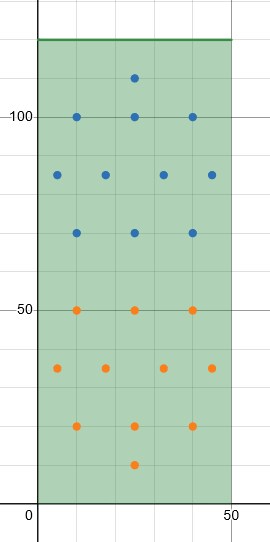
\includegraphics[width=0.5\textwidth]{images/field.png}
        \caption[The Playing Field]{The playing field is a rectangle of size 120yds by 50yds. Players are represented as points within the field.}
        \label{fig:field}
    \end{minipage}\hfill
    \begin{minipage}{0.45\textwidth}
        \centering
        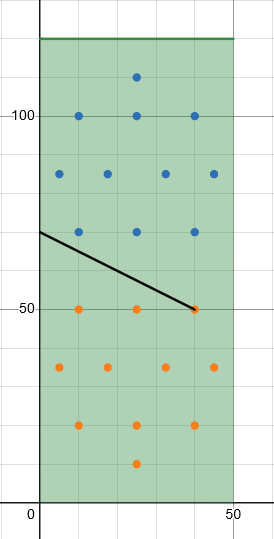
\includegraphics[width=0.5\textwidth]{images/ball path.png}
        \caption[The Ball Path]{The path of the ball represented by the parametric equation \(b(t)=(-2t+40,t+50)\).}
        \label{fig:ball-path}
    \end{minipage}
\end{figure}

\subsection*{The Ball}
At time \(t\), \(x(t)\) and \(y(t)\) will be the position of the ball on the \(x\) and \(y\) axes respectively. The path of the ball will be given by the parametric equation:
\begin{equation}
    b(t) = (x(t),y(t))
\end{equation}
The ball will always start its path from one of the players, \((x_s, y_s) = p_s \in P\). Therefore, \(x(t)\) and \(y(t)\) can be given by the following equations:
\begin{align*}
    x(t) &= a \cdot t + x_s \\
    y(t) &= b \cdot t + y_s
\end{align*}
where \(a\) and \(b\) are the ball's speed across each axis in \(yds/sec\). An example pass is shown in Figure~\ref{fig:ball-path}.

\begin{figure}[h]
    \centering
    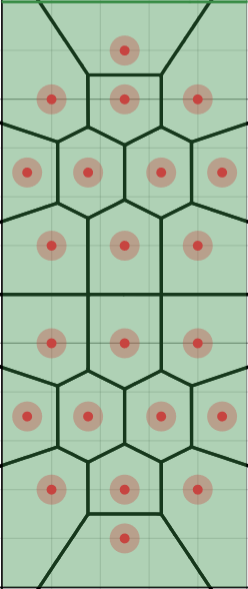
\includegraphics[width=0.25\textwidth]{images/voronoi.png}
    \caption{Voronoi Diagram of the Field}
    \label{fig:voronoi}
\end{figure}

\subsection*{The Diagram}
The Voronoi diagram of \(P\) is a partition of \(S\) into regions \(V(p_i)\) such that for each \(p_i \in P\), \(V(p_i)\) is the set of all points in \(S\) that are closer to \(p_i\) than
any other point in \(P\). We can use Fortune's algorithm to construct the Voronoi diagram in \(O(n \log n)\) time and \(O(n)\) space~\cite{fortune1987}.
An example diagram is shown in Figure~\ref{fig:voronoi}.

\begin{equation}
    V(p_i) = \{q \in S \ |\ \forall p_j \in P, d(p_i,q) \leq d(p_j,q)\}
\end{equation}

\section*{Determining the Receiver}
Now that we've constructed our Voronoi diagram and have a path for the ball, we can determine which player will receive the ball first. We will follow the ball through each Voronoi cell and,
as it exits the cell, we will check if the player in that cell can reach it before it exits. Since we know which player starts with the ball, we won't have to find the starting cell for the ball.
(Although we could do so in \(O(log(n))\) time using the trapezoidal-map search described by Hemmer, Kleinbort, and Halperin~\cite{hemmer2014optimal}.)
The cell the ball is currently in will be denoted by \(p_c\) which will be initialized to \(p_s\).
Our algorithm will have the following steps:

\begin{enumerate}
    \item Find the exit edge and exit time.
    \item Check if the player in the current cell can reach the ball before it exits.
    \item If the player can reach the ball, return the time and point at which they will receive it.
    \item If the player cannot reach the ball, move to the next cell.
    \item If the ball reaches the edge of the field, it is out of bounds and no player will receive it.
\end{enumerate}

\subsection*{Exit Edge and Time}
We iterate through every edge of the Voronoi cell and check if the ball's path intersects the edge. Assume that we are considering edge
\(e_{ij} = (v_i, v_j)\) where \(v_i\) and \(v_j\) are the vertices of the edge. The ball follows a parametric equation, so we'll convert the edge to a parametric equation as well.
First we calculate the rates of change across each axis:
\begin{align*}
    x_{\Delta} &= x_j - x_i \\
    y_{\Delta} &= y_j - y_i
\end{align*}
Then we plug the rates of change in with the starting point to get a parametric equation for the edge.
We use \(t_g\) as a placeholder to make the parametric equation, but this variable is only used when solving the system of equations since time isn't relevant for the edge.
\begin{equation}
    e_{ij}(t_g) = (x_{\Delta} t_g + x_i, y_{\Delta} t_g + y_i)
\end{equation}
We set the two equations equal to each other and solve for \(t_{exit}\). This will give us the time that the ball intersects the edge.
\begin{align*}
    b(t_{exit}) &= e_{ij}(t_g) \\
    a \cdot t_{exit} + x_s &= x_{\Delta} t_g + x_i \\
    b \cdot t_{exit} + y_s &= y_{\Delta} t_g + y_i
\end{align*}
If no answer exists, then the ball does not intersect the edge and we continue checking edges until we find one that intersects. Otherwise, we know that the ball crosses the edge at time \(t_{exit}\)
and we must check if the player in the current cell reaches the ball before it crosses.

\subsection*{Checking if the Player Intercepts the Ball}
To find an intersection between the player and the ball, we must first represent a feasible region for the player. This region will consist of all points that the player can reach
between the time the ball enters the cell and the time it exits. Given the player can travel in any direction at speed \(v\), the feasible region will be a circle with variable radius
\(r = v \cdot t_{c}\) where \(t_{c}\) is the current time.
It's possible that the player runs slower than \(v\), however, if the player has to run slower than \(v\) to reach the ball, then the player in the previous cell will always reach the ball first.
Therefore, we're only concerned about the player's feasible region between the time the ball enters the cell and the time it exits. We calculated \(t_{exit}\) in the previous step and
\(t_{enter}\) is initialized to \(0\) for the first cell, then set to the previous cell's \(t_{exit}\) for all subsequent cells.
\begin{equation}
    t_{enter} \leq t_c \leq t_{exit}
\end{equation}
With this information, we can represent the feasible region with the following parametric equation:

\begin{align*}
    c(t_g) &= (r cos(t_g) + p_x, r sin(t_g) + p_y) \\
    c(t_g) &= (v t_{c} cos(t_g) + p_x, v t_{c} sin(t_g) + p_y)
\end{align*}

Where \(p_x\) and \(p_y\) are the player's coordinates and \(t_g\) is another placeholder variable. We set the two equations equal to each other and solve the system of equations for \(t_c\):

\begin{align*}
    c(t_g) &= b(t_c) \\
    v t_{c} cos(t_g) + p_x &= a \cdot t_c + x_s \\
    v t_{c} sin(t_g) + p_y &= b \cdot t_c + y_s
\end{align*}

If no solution exists, then the player cannot reach the ball before it exits the cell and we move on to the next cell. Otherwise, we must confirm that at least one of the solutions is in the range
\(t_{enter} \leq t_c \leq t_{exit}\). If such a solution exists, then the player will receive the ball at time \(t_c\) and we can plug this time into \(b(t)\) to find the point of reception.
If all solutions are outside the range, then the player will not receive the ball and we continue to the next cell.

If we ever reach the edge of the field, then the ball is out of bounds and no player will receive it.

\section*{Complexity}
The complexity of this algorithm is \(O(n)\) where \(n\) is the number of players on the field. In the worst case, the ball passes through every cell and
we check every player for intersection with the ball. The check takes \(O(1)\) time and we perform it \(n\) times. In this case, we also check every edge for collision with
the path of the ball. Voronoi diagrams have no more than \(3n-6\) edges and the field adds no more than \(n + 4\) edges (one per cell plus one per corner).
Therefore, the worst case complexity is \(n + 3n - 6 + n + 4 = O(n)\).

\section*{Conclusion}
In this paper, we have described a method to utilize Voronoi diagrams to evaluate pass reception in sports. We construct a Voronoi diagram of the players on the field and then follow the ball
through each cell until we find a player that can receive it. This method is highly relevant to sports where players frequently pass the ball. A player, coach, or analyst could use this method
to analyze which passes are viable given the current positions of the players and which passes have no chance of success. There is still room to explore new methods and applications
of Voronoi and other dominant space diagrams for sports analysis and this paper is a step in that direction.

\subsection*{Future Work}
Any future works ought to consider a few variables that improve the realism of this process.
\begin{enumerate}
    \item Dominant regions. The dominant diagram takes into account the player's initial velocity and acceleration, and is therefore a more accurate representation of how a
    real player would move across the field.

    \item Unique player attributes. Some players might have faster acceleration and deceleration, some might have higher top speeds, and others might maintain speed while
    turning more efficiently. These attributes would need to be applied to each player in order to accurately evaluate who will receive the pass.

    \item The third dimension. This paper does not consider the possibility that the ball travels over the players' heads. Between adding an extra dimension to the Voronoi diagram,
    considering player height, and calculating ball trajectory, overhead passes become too complex a consideration for this paper.

    \item Higher complexity ball paths. The ball path in this paper is a simple linear parametric equation. In some sports, such as soccer, the ball can follow a curved path which may
    require additional considerations. In addition, a future method should consider that the ball loses speed over time.
\end{enumerate}
Due to time constraints, this paper was not able to take these factors into account.

\bibliography{references}{}
\bibliographystyle{plain}
\end{document}